\section{Implementation}

\subsection{Overview}
Since this section explains the current implementation of the developed tool set, it
not only aims to fulfill the dissertation's requirements, but also to help users
who want to understand the underlying systems and
prepare them for potentially joining the development effort. Although abridged code
extracts are of their current state for thesis submission, and the main
principles will remain, nevertheless future readers are welcome to consult the actual
source code if any discrepancies arise or reexport the document.

Firstly  the main libraries are briefly explained where they are relevant to the
program. Secondly, the mostly abstract plugin architecture is shown. Thirdly the main plugins are presented and last the
delivery processes to the end users are described.


All implementation files are contained and delivered inside a single git
repository, which is freely available online:
\url{https://github.com/ksjogo/oxrti}.
All following file paths are relative to that repository's root. All future development will
be immediately available there and the current compiled software version is
always fed automatically from it into the hosted version at \url{https://oxrtimaster.azurewebsites.net/api/azurestatic}.

\subsection{Libraries}
\subsubsection*{TypeScript}
 The official header line of TypeScript gives reasons why
  it was picked for this project: ``TypeScript is a typed superset of JavaScript that compiles
  to plain JavaScript. Any browser. Any host. Any OS\@. Open
  source.''\cite{noauthor_typescript_2018} Which fits
  requirements~\ref{req_os},~\ref{req_system}. Whereas plain JavaScript would
  have allowed slightly easier initial on-boarding and maybe easier immediate
  code `hacks', TypeScript will provide better stability in the long term and a
  quite improved developer experience (requirement~\ref{req_dx}) in the long
  run. With the full typed hook system (compare \autoref{sec_hooks}) it ensures
  that a compiled plugin will not have runtime type problems, reducing the
  amount of switching between code editor and the running software. The whole
  project is set up in a way to fully embrace editor tooling. Visual Studio
  Code\cite*{noauthor_visual_nodate} and Emacs\cite*{noauthor_gnu_nodate} are
  the `officially' tested editors of the project. Code is recommended as it will
  support all developer features out of the box. The installation of the
  tslint\cite*{noauthor_tslint_nodate} plugin\cite*{noauthor_tslint_nodate-1} is
  recommended to keep a consistent code style, which is configured within the
  \emph{tslint.json} file. Most importantly TypeScript adds type declarations
  (and inference) to JavaScript, e.g.:
\begin{typescript}
const thing = function (times: number, other: (index: number) => boolean) { ... }
\end{typescript}
would define \emph{thing} as a function, taking a numbers as first argument and
another function (taking a number as first parameter and returning a boolean) as
second argument. The other most used TypeScript features inside the codebase are
Classes\cite*{noauthor_classes_nodate},
Decorators\cite*{noauthor_decorators_nodate} and
Generics\cite*{noauthor_generics_nodate}, which will be discussed at their first
appearance inside the code samples.
\subsubsection*{React}
The two main points on React's official website are
  ``Declarative'' and ``Component Based''\cite*{noauthor_react_nodate}, which
  is best shown by an extended example from their website, which exemplifies
  multiple patterns found through the oxrti implementation. The most important
  concept is the jump from having a stateful HTML document, which the JavaScript
  code is manipulating directly, e.g.:
  \begin{typescript}
document.getElementById('gsr').innerHTML="<p>You shouldn't do this</p>"
\end{typescript}
Which is diametric to requirements~\ref{req_easy} and~\ref{req_dx} as it would
require developers to manually keep track of all data cross-references (e.g.\
the pan values having to automatically adapt to the current zoom level). A
declarative approach instead allows much better and easier implemented
reactiveness and better performance (requirements~\ref{req_performance}
and~\ref{req_react}) as the necessary changes can be tracked and components can be
updated selectively.

\begin{typescript}
// a class represents a single component
class Timer extends React.Component {
  // the parent component can pass on props to it
  constructor(props) {
    super(props);
    this.state = { seconds: 0 };
  }

  tick() {
    //  the state is updated and the component is automatically re-rendered
    this.setState(prevState => ({
      seconds: prevState.seconds + 1
    }));
  }

  // called after the component was created/added to the browser window
  componentDidMount() {
    this.interval = setInterval(() => this.tick(), 1000);
  }

  // called before the component will be deleted/removed from the browser window
  componentWillUnmount() {
    clearInterval(this.interval);
  }

  // the actual rendering code
  // html can be directly embedded into react components
  // {} blocks will be evaluated when the render method is called
  // which will happen any time the props or its internal states updates
  render() {
    return (
      <div>
        Seconds: {this.state.seconds}
      </div>
    );
  }
}

// mountNode is a reference to a DOM Node
// the component will be mounted inside that node
ReactDOM.render(<Timer />, mountNode);
\end{typescript}
In conjunction with mobx and TypeScript no classes are used for React components
though, but instead Stateless Functional Components
(`SFCs'\cite*{ikeuchi_react_2017}). These SFCs are plain functions, only
depending on their passed properties:
\begin{typescript}
function SomeComponent(props: any) {
 return <p>{props.first} {props.first}</p>
}
\end{typescript}
This component could then be used by:
\begin{typescript}
 <SomeComponent first="Hello" second="World"/>
\end{typescript}
This component systems allows the plugins to define some components and then
`link' them into the program via the hook system, which will be explored later.
\subsubsection*{MobX}
Its main tagline is ``Simple, scalable state
  management''\cite*{noauthor_mobx:_2018}. An introductory overview is shown
  in~\autoref{mobxflow}. Broadly speaking MobX introduces observable objects.
  Instead of the aforementioned DOM handling or property passing inside React trees,
  components can just retrieve their values from the observable objects and will
  be automatically refreshed if the read values change. This for example makes
  the implementation of the QuickPan plugin extremely easy, as it can just read
  the zoom, pan, etc.\ values of the other plugins and will automatically receive
  all updates without any further manual observation handling.
  \sidefig{mobxflow}{MobX Flow}{Taken from
    Weststrate\cite*{noauthor_mobx:_2018}. Actions in the oxrti context are most
  often initially user actions, which are then calling into plugins to change
  the state. The state is mostly encapsulated on a plugin basis with usage of
  the mobx-state-tree library, which also encapsulates most computed values.
  Reactions are most often the previously discussed React components.}
\subsubsection*{mobx-state-tree}
``Central in MST (mobx-state-tree) is the concept of a
  living tree. The tree consists of mutable, but strictly protected
  objects''\cite*{noauthor_mobx-state-tree:_2018} This allows the implementation
  to have one shared state tree which can be used to safely access all data. All
  nodes inside the state tree are MobX observables. A simple tree with plain MST
  would look like this:
\begin{typescript}
// define a model type
const Todo = types
 .model("Todo", {
  // state of every model
  title: types.string,
  done: false
 })
 .actions(self => ({
  //methods bounds to the current model instance
  toggle() {
   self.done = !self.done
  }
 }))
// create a tree root, with a property todos
const Store = types.model("Store", {
    todos: types.array(Todo)
})
\end{typescript}
This syntax was deemed to convoluted, as it is a lot more complex than standard
JavaScript/TypeScript classes, which were introduced by the ES6 version, as shown in the React description above and
thus being in conflict with requirement~\ref{req_easy}.
\subsubsection*{classy-mst}
There is an option to use a more traditional syntax instead
  though, with the classy-mst library, with
  which the example above becomes\cite*{noauthor_classy-mst:_2018}:
\begin{typescript}
const TodoData = types.model({
	title: types.string,
	done: false

});

class TodoCode extends shim(TodoData) {
	@action
	toggle() {
		this.done = !this.done;
	}
}

const Todo = mst(TodoCode, TodoData, 'Todo');
\end{typescript}
 Weststrate, the original author of MobX initially was sceptic of this
 syntax\cite*{noauthor_alternative_nodate} as it was changing the semantics of
 ES6 classes, as classy-mst's methods will be automatically bound to the
 instance. This boundness is an advantage for this implementation though, as the
 hook configurations can just refer to \code{this.someMethod} instead of \code{this.someMethod.bind(this)}.
The \code{@action} is a decorator, enabling the following method to change the
state/properties of the model, as MST prohibits that by default. Reactions/View
updates will only happen after the outermost action finished executing.
\subsubsection*{WebGL}
The increasing support of the WebGL stack is the main reason why
  it is now feasible to implement a full RTI software stack with plain web
  technologies, as it ``enables web content to use an API based on OpenGL ES 2.0
  to perform 3D rendering in an HTML \code{<canvas>} in browsers that support it
  without the use of plug-ins."\cite*{noauthor_webgl_nodate-1} OpenGL ES 2.0
  likeness means that (most importantly) shaders are supported, allowing the
  implementation to be split up into multiple shaders with single
  responsibilities. For details refer to~\autoref{sec_rendererstack}. While preserving compatibility and
  requirement~\ref{req_system} WebGL 2 support is sadly not widespread enough to fully rely on yet
  (compare~\autoref{webglcomp}), as it is currently estimated at 50\% of all devices\cite*{noauthor_webgl_nodate-2}.
  \fig{webglcomp}{WebGL compability}{WebGL compability as from the Mozilla
    Developer network\cite*{noauthor_webgl_nodate}.}  Potential improvements
  when WebGL 2 is more widely supported or in conditional plugins are discussed
  in~\autoref{sec_future}. One notable limitation of WebGL is
  \code{MAX_TEXTURE_IMAGE_UNITS}, the maximum amount of bound textures inside a
  single shader, which in most implementations is
  16\cite*{noauthor_webgl_nodate-3}, whereas the standard OpenGL implementations
  are likely to have a limit of 32. This is influencing the BTF file format, as
  for example in the PTM RGB use case a total of 18 coefficients exist, which
  now need to be bundled up somehow into maximum 16 textures, if the
  calculations should be done inside a single shader. It is also limiting the
  amount of layers of the Paint plugin, as these also consist of bound textures.
  Apart from the shaders, which are written in the OpenGL ES
  Shading Language\cite*{noauthor_webgl_nodate-4} and the the texture loader (\autoref{sec_textureloader}), no direct
  WebGL code is necessary nor used anywhere inside the implementation, as the
  gl-react library is abstracting it neatly for use from the MobX/React environment.

  \subsubsection*{gl-react}
 ``Implement complex effects by composing React
  components.''\cite*{renaudeau_gl-react_2018} is the main use of the gl-react
  library. A minimal component, adapted from the gl-react-cookbook looks
  like\cite*{renaudeau_gl-react_2018}:
\begin{typescript}
const shaders = Shaders.create({
  helloGL: {
    frag: GLSL`
     precision highp float;
     varying vec2 uv;
     void main() {
      gl_FragColor = vec4(uv.x, uv.y, 0.5, 1.0);
   }`
 }
});

export default class Example extends Component {
  render() {
    return (
      <Surface width={300} height={300}>
        <Node shader={shaders.helloGL} />
      </Surface>
    );
  }
}
\end{typescript}
  Which would result in a display like~\autoref{glreactcookbook}.
  \fig{glreactcookbook}{gl-react-cookbook example}{RGBA texture, with R and G
    according to their respective u or v texture coordinate. From
    \cite*{noauthor_gl-react_nodate}.} gl-react's is not a 3D engine, so no
  objects are to be created or scene graph managed, instead the oxrti
  implementation can concentrate on solely providing the necessary shaders.\
  gl-react's default node size is taken from the parent surface size. The
  surface size will be dependent on the user running the program and his browser
  windows, which makes it undesirable as details would be lost, if the BTF
  provided more detail, so the processing Node sizes are usually set to the BTF
  resolution or higher.
  \subsubsection*{Webpack}
  Webpack is used to bundle the implementation into single files as it is ``a bundler for javascript and friends. Packs many modules into a few bundled
  assets.''\cite*{noauthor_webpack/webpack:_nodate} A more detailed discussion
  on the targets is in~\autoref{sec_apps}. Broadly speaking Webpack loads the
  source code inside the \emph{src} directory according to the loaders defined
  inside the \emph{webpack.config.js} file, analyses their dependencies and then
  bundles them together. This makes it possible to have a dependency tree
  spanning 26184 packages from npm, but still providing a single bundled
  application file only 1.5 megabyte large (data as of \today). It also allows
  the dynamic plugin structure by bundling the plugins into a dynamic `context' from
  which single plugins can be loaded at runtime.
  \subsubsection*{Electron}
  Electron is used to ``build cross-platform desktop apps with JavaScript, HTML,
  and CSS''\cite*{noauthor_electron:_2018} While theoretically not necessary to
  fulfill most requirements, as the implementation is compatible with all modern
  web browsers, an additional standalone executable provides some advantages:
  \begin{itemize}
\item It is possible to add a more traditional menu-based interface, which the
  browser version could not support.
  \item Stable development environment, as electron-devtools-installer is used
    to provide relevant extensions (React devtools, MobX devtools) by default
    and the hot reloading is reliably tested, which together form a good
    developer experience (requirement~\ref{req_dx})
  \item It allows to preserve the software in a usable, contained state, not
    relying on the user also having a compatible web browser in the future.
\item It allows future development to more directly access resources of the host
  machine, e.g.\ the normal OpenGL stack could be used for calculating the
  coefficients, as it is less resource constrained compared to the WebGL stack.
  \end{itemize}
  \subsubsection*{MaterialUI}
  MaterialUI is succinctly described by ``React components that implement
  Google's Material Design.''\cite*{noauthor_material-ui:_2018}. MaterialUI's
  component are used throughout the app for styling the components, making the
  use of custom CSS largely unnecessary apart from minor positioning fixes. For
  example the Zoom component is defined as:
\begin{typescript}
// Card, CardContent, Tooltip and Button are all components provided by MaterialUI.
// this refers to the Zoom Plugin's controller which
// the content will be automatically refreshed if the refered values change
const Zoom = Component(function ZoomSlider (props) {
    return <Card style={{ width: '100%' }} >
        <CardContent>
            <Tooltip title='Reset'>
                <Button onClick={this.resetZoom} style={{ marginLeft: '-8px' }}>Zoom</Button>
            </Tooltip>
            <Tooltip title={this.scale}>
                <Slider value={this.scale} onChange={this.onSlider} min={0.01} max={30} />
            </Tooltip>
            <Tooltip title='Reset'>
                <Button onClick={this.resetPan} style={{ marginLeft: '-11px' }}>Pan</Button>
            </Tooltip>
            <Tooltip title={this.panX}>
                <Slider value={this.panX} onChange={this.onSliderX} min={-1 * this.scale} max={1 * this.scale} />
            </Tooltip>
            <Tooltip title={this.panY}>
                <Slider value={this.panY} onChange={this.onSliderY} min={-1 * this.scale} max={1 * this.scale} />
            </Tooltip>
        </CardContent>
    </Card>
})
\end{typescript}
It would result in a display like~\autoref{zoomcomponent}.
\fig{zoomcomponent}{Zoom Component}{Zoom Component, the user is dragging the
  zoom slider currently, the mouse pointer is not depicted.}
 \subsubsection*{Misc}
 Further libraries of note are:
\begin{description}
\item[electron-webpack\cite*{noauthor_electron-userland/electron-webpack:_nodate}] is providing the bridging between Webpack and
   Electron, its config is expanded by the \emph{webpack.renderer.additions.js}
   and \emph{webpack.renderer.shared.js} files.
\item[pngjs\cite*{stolwijk_pngjs:_2018}] is providing in-browser bitwise png
  manipulation, required in the converter.
\item[jszip\cite*{noauthor_jszip_nodate}] is providing in-browser zip file
    manipulations, which are fundamental for the BTF fileformat.
\end{description}


\subsection{Base}
The implementation is making a distinction between plugin and non-plugin files.
The amount of non-plugin files was aimed for to be as low as possible, as they
are inflexible in all output configurations and will have slightly different
behaviour while developing in regard to reloads. The files not contained in
plugins are the following:
\begin{itemize}
\item \emph{AppState.tsx}, the mobx-state-tree root node representing the whole
  application state in its leafs, detailed in~\autoref{sec_state}.
 \item \emph{BTFFile.tsx}, containing the fileformat implementation and utility
   functions, described in~\autoref{sec_btffile}.
\item \emph{Hook.tsx} and \emph{HookManager.tsx} which provide the whole dynamic
  interaction system between the different plugins, shown
  in~\autoref{sec_hooks}.
\item \emph{Loader.tsx}, \emph{electron/index.tsx}, \emph{renderer/index.tsx}
  and \emph{web/index.tsx}, providing the loading functionality. The Electron
  application has two entry points, one for the main process, which is
  \emph{electron/index.tsx} and one for the in-browser content, which is
  \emph{renderer/index.tsx}. The in-browser one and the plain browser entry point
  \emph{web/index.tsx} both call the \emph{Loader.tsx} to initialise the state
  management and mount the root React component, so the user can interact
  finally. The Loader also handles hot-reloading, it will receive the changed
  source code from Webpack and update the plugins accordingly.
 \item \emph{Plugin.tsx} defining the base class for a plugins, further
   explained in~\autoref{sec_plugins}.
\item \emph{types.d.ts} is providing the custom ambient type declarations for
  software dependencies, which are not providing TypeScript types on their own.
  In case new dependencies are added, they are likely to require and addition there.
\item \emph{Util.tsx} providing general helper functions, largely related to
  some math functions for texture coordinate handling.
\item \emph{loaders/glslify-loader/index.js} is the custom Webpack loader for
  \emph{.glsl} files, allowing e.g.\ the \code{import zoomShader from
    './zoom.glsl'} statement and setting up Webpack to contain the shader source
  in the final bundle.
\item \emph{loaders/oxrtidatatex/OxrtiDataTextureLoader.tsx} is providing direct
  texture loading from in-memory BTF files, discussed in~\autoref{sec_textureloader}.
\end{itemize}

\subsection{Hooks}\label{sec_hooks}
The hook system allows stable and prioritized interactions between the different
plugins. All available hooks are declared inside the {Hook.tsx} file, which
offers 3 different types of hooks:
\sourceBE{Hook.tsx}
These types are used to first declare single hook types (which will be discussed
within the plugins consuming them) and then construct the whole hook
configuration tree for all plugins:
\begin{typescript}
type HookTypes = {
  ActionBar?: ConfigHook<ActionBar>,
  AfterPluginLoads?: FunctionHook,
  AppView?: ComponentHook,
...
}
\end{typescript}
A plugin then can link itself into these hooks with its hooks method, for
example:
\begin{typescript}
get hooks () {
  return {
    // register things for the ViewerSide hook / add components to the side bar
    ViewerSide: {
      // a plugin can register itself multiple times with different names and configurations
      Metadata: {
        component: BTFMetadataConciseDisplay,
        // hooks will be sorted internally in priority order, highest first
        priority: -110,
      },
      Open: {
        component: Upload,
        priority: 100,
      },
    },
  }
}
\end{typescript}
The state manager (~\autoref{sec_state}) collects all hooks and merges them into
the respective HookManagers, which are then used to iterate/map over these hooks
with 4 convenience functions \code{forEach}, \code{asyncForEach},
\code{forEachReverse}, \code{map} and \code{pick}.

\subsection{BTF File}\label{sec_btffile}
The full standalone BTF file format specification can be found inside~\autoref{sec_fileformat}.
The implementation in \emph{BTFFile.tsx} is an in-memory implementation of that
file with following interface, it is mainly a `dumb' data container.
\desc{beginBTF}{endBTF}{BTFFile}
Notable is the \code{PreDownload} hook which is called before the
\code{generateZip} function is called, to allow the ImpExp plugin and the Paint
plugin to fill the BTF with their respective data. This hook is called by the
AppState though, as the BTFFile implementation is fully standalone (apart from
the jszip dependency), in case other software wishes to re-use the implementation.


\subsection{State Management}\label{sec_state}
The \emph{AppState.tsx} file is the root of the applications state tree, but
itself only contains limited data:
\source{beginData}{endData}{AppState.tsx}
Its main function is to load all plugins and then let them share data between
each other via the hook system. The set of plugins to be loaded is defined inside
\emph{oxrti.plugins.json}, the plugins defined there will be loaded in order.
The state tree after inital plugin load is shown in~\autoref{statetree}.
As only \code{@action}s can modify the state, it is easy to follow the changing
app state, as shown in~\autoref{mobxactions}.
\fig{mobxactions}{MobX actions}{Run MobX at application startup and after one
  click on `Add Bookmark'. The differential of that action is on the right.}
\fig{statetree}{MobX state tree}{State tree after inital application load. All
  plugins are initialized and their hooks are registered. Visualized with redux
  dev tools.\cite*{noauthor_redux_nodate}}

\subsection{Renderer Stack}\label{sec_rendererstack}
Even though the renderer stack is fully contained in the plugins, its principles
span most of them, thus an overview is in order. All WebGL rendering is done
through the gl-react library. If a plugin wants to register a node inside the
stack, it is using the hook system, e.g.\ the Rotation plugin:
\source{beginRotationHooks}{endRotationHooks}{Plugins/RotationPlugin/RotationPlugin.tsx}
The registered nodes are components again, which will link them into the
automated mobx reactions, for example the Centerer node:
\source{beginCenterer}{endCenterer}{Plugins/RotationPlugin/RotationPlugin.tsx}
For the currently delivered default configuration the following nodes are
registered:
\begin{enumerate}
\item PaintNode
\item CentererNode
\item RotationNode
\item ZoomNode
\end{enumerate}
The Renderer plugin will start by picking the proper base rendering node
depending on the channel format of the currently loaded BTF file (btf inside the
code):
\source{beingPicker}{endPicker}{Plugins/RendererPlugin/RendererPlugin.tsx}
This inital node will then be wrapped by the registered nodes:
\source{beingWrapper}{endWrapper}{Plugins/RendererPlugin/RendererPlugin.tsx}

\subsection{Texture Loader}\label{sec_textureloader}
The bridge between the loaded BTF files and the WebGL contexts needs to be
closed with custom code, as gl-react was not supporting the load of PNG textures
from memory. An abridged version of the code follows, as it is a good example of
the Promise pattern used in some following parts.
\begin{typescript}
loadTexture(config: TexForRender) {
    // keep track of the amount of currently loading textures
    appState.textureIsLoading()
    // shortcut for the WebGL reference
    let gl = this.gl
    // access the raw data buffer from the texture configuration
    let data = config.data
    // create a Promise, that basically is chaining callbacks together and then asynchronously executing each step
    let promise =
        // first create an ImageBitmap object, we need to flipY as the textures
        are orientated naturally inside the BTF file but WebGL is expecting them bottom row first
        createImageBitmap(data, { imageOrientation: 'flipY' })
        // the catch step is called if the previous part failed
        .catch((reason) => {
            // some browsers do not like loading a lot of big textures in parallel and will garbage collect them in between and thus fail, as a fallback the limiter function is used to limit concurrency of that part
            return limiter(() => createImageBitmap(data))
        })
        // the then part is called when the previous step succeeded
        .then(img => {
            // create and bind a new WebGL texture
            let texture = gl.createTexture()
            gl.bindTexture(gl.TEXTURE_2D, texture)
            let type: number
            // map the type from the BTF file to a WebGL texture type
            switch (config.format) {
                case 'PNG8':
                    type = gl.LUMINANCE
                    break
                // ...
                case 'PNG32':
                    type = gl.RGBA
                    break
            }
            // load the imageBitmap into the texture
            gl.texImage2D(gl.TEXTURE_2D, 0, type, type, gl.UNSIGNED_BYTE, img)
            gl.texParameteri(gl.TEXTURE_2D, gl.TEXTURE_MIN_FILTER, gl.NEAREST)
            gl.texParameteri(gl.TEXTURE_2D, gl.TEXTURE_MAG_FILTER, gl.NEAREST)
            // finished and return
            appState.textureLoaded()
            return { texture, width: img.width, height: img.height }
        })
        .catch((reason) => {
            // a null texture will be empty
            alert('Texture failed to load' + reason)
            appState.textureLoaded()
            return { texture: null, width: config.width, height: config.height }
        })
   // the calling code will have its own catch/then logic
   return promise
}
\end{typescript}

\subsection{Plugins}\label{sec_plugins}
All plugins extend the relatively limited abstract plugin class in
\emph{Plugin.tsx} and have no preserved state:
\descBE{Plugin}
The most important function is the \code{PluginCreator}, which merges the
mobx-state-tree model with the classy-mst controller code and provides a wrapper
function to create components bound to the containing plugin:
\source{beginCreator}{endCreator}{Plugin.tsx}
A minimal example would be:
\sourceBE{Plugins/BasePlugin/BasePlugin.tsx}
The rest of the plugins are presented on a higher conceptual level, as their
internal APIs are most times used only by themselves. Their hooks will be
discussed though.

\subsubsection{Base Plugin}
The base plugin is containing no further internal logic, but only is providing
some shared display components. These could theoretically have been implemented
outside of any plugin, but putting them into the Base plugin simplifies the
distinction between components bound to plugins and unbound plugins, by having
no unbound plugins at all. It also simplifies the code loading, as just the Base
plugin can be (re-)loaded like all other plugins. The provided components are:
\begin{itemize}
\item JSONDisplay, showing a JSON object in a prettified form, used for
  displaying different metadata objects
\item BTFMetadataDisplay, showing the currently loaded BTF's data
\item RenderHooks, to render all components attached to a hook
\item SafeGLIInspector, wrapping the secondary WebGL surfaces and disabling
    theme, if WebGL debug tools are used, which can handle only one surface.
\item Tooltip, wrapping the material-ui tooltip component to fix styling errors
\end{itemize}

\subsubsection{BaseTheme, RedTheme and BlueTheme Plugin}
The BaseTheme plugin is having two essential properties:
\code{themeBase} and \code{themeExtension}. \code{themeBase} contains the app
wide configuration for the MaterialUI library.Concrete themes (at the moment RedTheme and BlueTheme plugins) extend this
BaseTheme and then set their \code{themeExtension} according to their
modifications. To pick a theme to be used the ThemeConfig hook exists:
\source{ThemeHooksBegin}{ThemeHooksEnd}{Hook.tsx}
Concrete themes register with:
\sourceBE{Plugins/RedThemePlugin/RedThemePlugin.tsx}
If multiple plugins are registering themes, the appState will pick the theme
with the highest priority to apply to the app.

\subsubsection{TabView Plugin}
The TabView plugin is providing the full app experience and is targeted at the
Electron output and the online hosted version. As a tabbed container will
occasionally delete the content of non-active tabs, some hooks are needed to
ensure graceful behaviour of all displayed tabs:
\source{AppHooksBegin}{AppHooksEnd}{Hook.tsx}
This view is depicted in~\autoref{viewcomparison}.

\subsubsection{SingleView Plugin}
The SingleView plugin is aimed to provide a contained viewer experience, e.g.\ on
a museum's website, it is just displaying the tab with the highest priority, see~\autoref{viewcomparison}.

\begin{figure}
  \begin{subfloat}[Viewer with TabView and RedTheme]
    {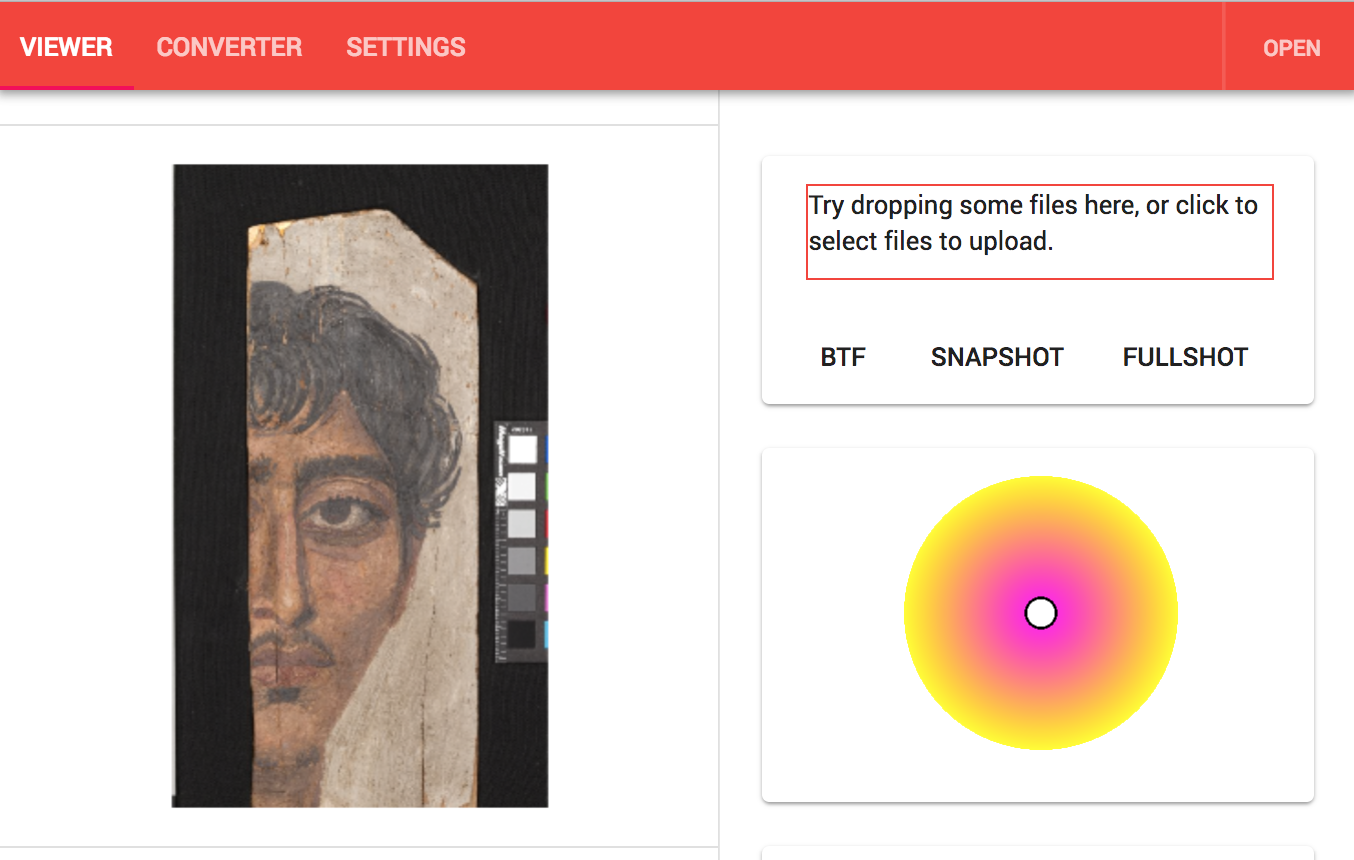
\includegraphics[max
    width=0.5\linewidth]{images/tabview}}
\end{subfloat}
\begin{subfloat}[Viewer with SingleView and BlueTheme]
  {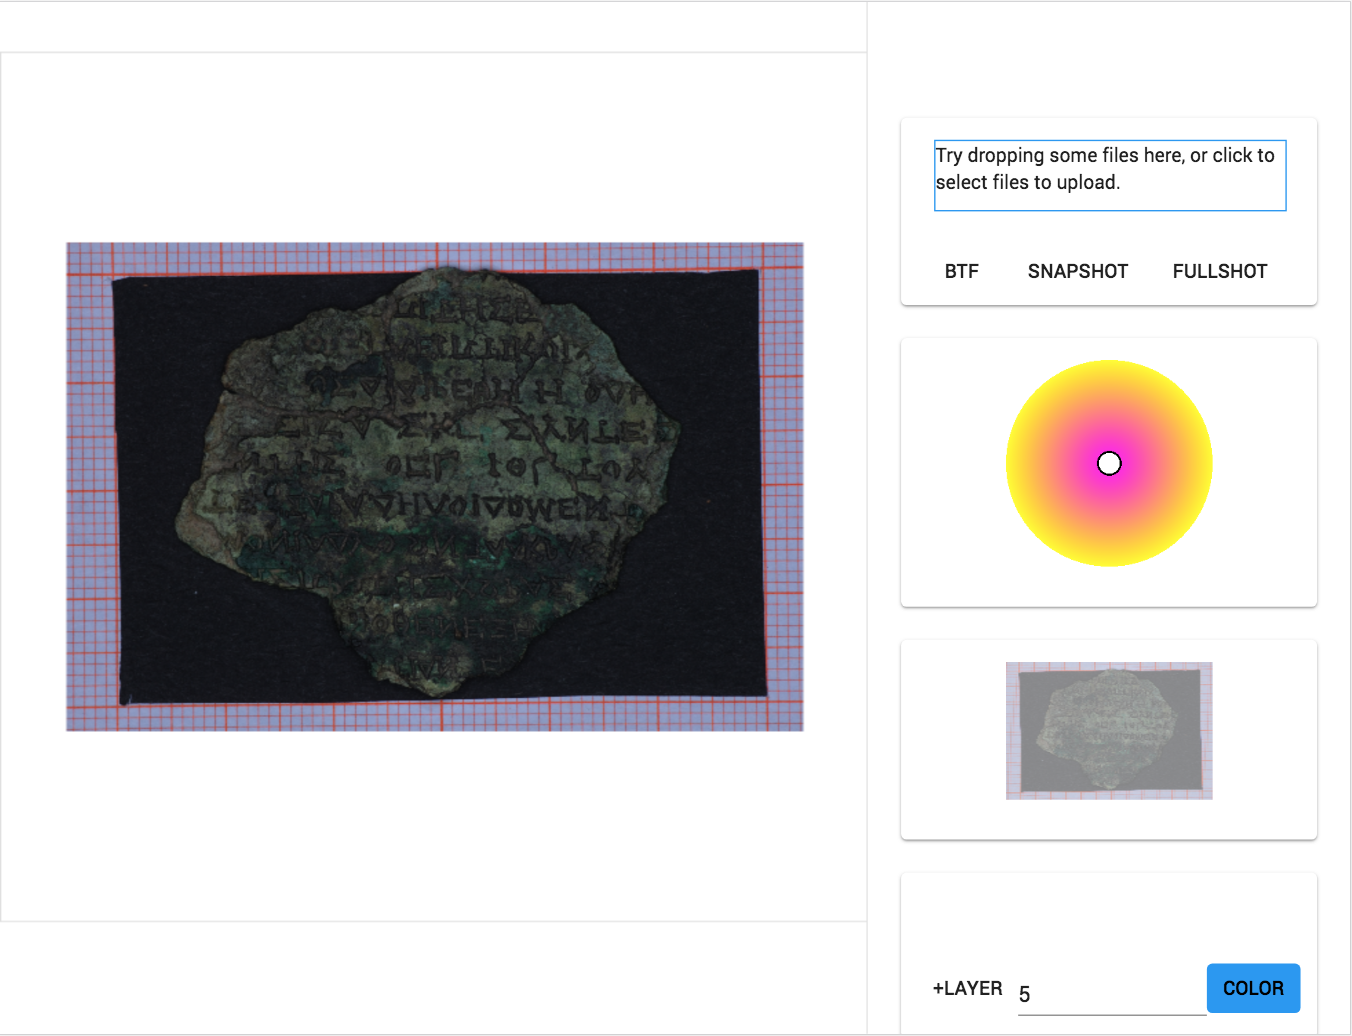
\includegraphics[max
    width=0.5\linewidth]{images/singleview}}
\end{subfloat}
\caption[View Comparison]{Only changes are two lines in \emph{oxrti.plugins.json}.}
\label{viewcomparison}
\end{figure}


\subsubsection{Converter Plugin}
The Converter plugin consists of multiple parts:
\begin{itemize}
\item The converter user interface, as shown in~\autoref{converterui}.
\item BMPWriter and PNGWriter, both extending Writer to write the converted
  textures. The BMPWriter is customised as no current package is offering the
  required functionality. The PNGWriter is wrapping pngjs.
\item An abstract base converter strategy, to be extended by plugins providing a
  concrete converter with the following interface:
\end{itemize}
\fig{converterui}{Converter UI}{Converter user interface, with display of the
  extract manifest.}
\descBE{Plugins/ConverterPlugin/ConverterStrategy}
If a plugin wants to register a concrete converter it would use following hook:
\sourceBE{Plugins/PTMConverterPlugin/PTMConverterPlugin.tsx}

\subsubsection{PTMConverter Plugin}\label{sec_ptmconverter}
The PTM Converter plugin is converting \emph{.ptm} files, as they are described
in~\autoref{sec_relfile}. Currently the RGB and LRGB light models are
supported. They main interesting part is the pixel data reader:
\source{beginRead}{endRead}{Plugins/PTMConverterPlugin/PTMConverterStrategy.tsx}

\subsubsection{Renderer Plugin}
The Renderer plugin is providing the main user interface, which is split into
two parts, on the left the rendered object and on
the right further controls. As such it is using a comprehensive set of hooks:
\source{RendererHooksBegin}{RendererHooksEnd}{Hook.tsx}
The actual object rendering is done by the stack as described
in~\autoref{sec_rendererstack}, the Renderer plugin is only providing a
dynamically resized and centered surface for the stack to be drawn in. The
surface is always kept square, even if the loaded BTF is not, to streamline and
simplify texture coordinate handling.

\subsubsection{PTMRenderer Plugin}\label{sec_ptmrender}
The PTMRenderer Plugin is rendering the RGB and LRGB channel
models. Here only the RGB is covered, as the principles for LRGB are the same.
Most channel renderers will be split in two parts, one node for the rendering
stack:
\sourceBE{Plugins/PTMRendererPlugin/PTMRendererPlugin.tsx}
And one shader, implementing the light model described in~\autoref{sec_relfile}.
\glsl{Plugins/PTMRendererPlugin/ptmrgb.glsl}
In addition to the default rendering mode the PTMRenderer plugin is also
supporting a Normals rendering mode for LRGB ptms. See~\autoref{renderingmodes}
for a visual example. It is based on the proposal by MacDonald and
Robson\cite*{macdonald_polynomial_2010} and currently supports 4 extra rendering
modes: X-Normal, Y-Normal, Z-Normal and False-Color-Normal. The first three
render the respective value of the normal of the pixel as grey scale, the false
color one maps X to R, Y to G and Z to B.
\fig{renderingmodes}{Normal Rendering}{The Tablet ptm rendered with false color
  normals. The user can change the mode with the `Rendering Mode'' drop down on
  the top right.  }

\subsubsection{LightControl Plugin}
The LightControl plugin is providing a visual way to control the position of the
light source. The user interface is shown in~\autoref{lightcontrol}. The
linear xy coordinates are transformed into hemispherical coordinates, which are
then passed onto the current Base node from the Renderer plugin.
\fig{lightcontrol}{LightControl Plugin}{The user can drag around on the imaginary
  dome and change the light position.}

\subsubsection{Rotation Plugin}
The Rotation plugin allows the rotation of the viewed object (and other lower
rendering nodes). It does so by first centering the object inside a large square
node of the maximal spanning length when rotated ($width * Math.cos(Math.PI / 4) + height * Math.sin(Math.PI /
  4)$), so no part will be cut off for the rendering layers on top, and then
applying a simple rotation matrix on the texture coordinates on the next node. Even though the whole
renderer is rotated, the use of rotation slider will dynamically adapt the pan
values to keep the previous center centered.

\subsubsection{Zoom Plugin}
The Zoom plugin is providing zoom and pan functionality (pan would not be
necessary without zoom), an example is~\autoref{zoom}. All zooming and panning
is implemented as a special shader in the render stack.
\fig{zoom}{Zoom Plugin}{Applied zoom, note the small part of the actual object
  being shown. The shader architecture allows for seamless and performant
  zooming between nearest viewpoints and more removed ones. }

\subsubsection{QuickPan Plugin}
The QuickPan plugin is responsible for rendering the small view box on the top
right inside~\autoref{zoom}. It is doing so by
rendering injecting a temporary node inside the rendering stack, waiting for an
object's first render and then preserving that texture in a lower resolution, by setting the \code{width} and \code{height} properties of
the nodes (compare the component in~\autoref{sec_ptmrender}). It then uses the
RectRender component to render the semi-transparent rectangle of the current
visible part over the captured texture. To do so, it is using the \code{inversePoint} function on \code{[0, 0]},
\code{[0,1]}, \code{[1,1]}, \code{[0,1]} to transform the bounds of the
currently rendered (main) surface into texture coordinates of the object. With
these coordinates a simple point-in-rectangle check can be done to highlight the
desired area.

\subsubsection{Paint Plugin}
The Paint plugin adds the functionality to have overlays on the object to allow
for annotations in a research context. All painting is happening as part of the
renderer stack, with one node for each layer and one mixer node to combine these
with the object. One interesting point is the required recompilation of the
mixer shader,  as the WebGL compiler is not supporting loops with unfixed
amounts of maximal iterations. So for each new layer the shader source is changed.
%As the Paint plugin is interesting in terms of implementation, it is
%presented in more detail. The main Paint node:
%\sourceBE{Plugins/PaintPlugin/PaintPlugin.tsx}
%The shaders are comparatively simple. Paint first:
%\glsl{Plugins/PaintPlugin/paint.glsl}
%\source{beginMixerShader}{endMixerShader}{Plugins/PaintPlugin/PaintPlugin.tsx}
%Mixer source:
%\glsl{Plugins/PaintPlugin/mixer.glsl}
The user interface is shown in~\autoref{painting}. Up to 15 layers are supported
currently, as the max texture limit is usually 16.
\fig{painting}{Paint Plugin}{Paint plugin user interface. The check mark in
  front indicates the layer is currently drawn on. Names are freely changeable.
  The toggle toggles visibility of the layer. The trash icon deletes the
  corresponding layer. +Layer adds another layer on top. The number is the brush
size. Clicking color shows a color picker.}

\subsubsection{Bookmarks Plugin}
The Bookmarks plugins allows bookmarks to be set for light and view
configurations. Bookmarks are controlled via the following hook:
\source{BookmarkHooksBegin}{BookmarkHooksEnd}{Hook.tsx}
\fig{bookmark}{Bookmark Plugin}{A click on `Add Bookmark' will preserve the
  current light and camera positions and create an unnamed entry in the bookmark
list. Clicking `RES' restores this configuration. They are automatically
exported when saving the current BTF.}

\subsubsection{Notes Plugin}
The Notes plugin implements notes, which are attached to a specific point of the
viewed object. Each note consists of two parts: One indicator which is linked
to the texture and whose position is transformed like the texture and one popup,
which calculates its absolute screen coordinates to show the note's name and
text. See~\autoref{notes} for an example.
\fig{notes}{Notes Plugin}{Notes are created by switching the `Notes Create:'
  toggle and then clicking anywhere on the texture. The red and white dots
  indicate the presence of a note at that point, clicking it will toggle the
  display of the note. Clicking the note's name on the right side, will center
  that note's indicator.}

\subsubsection{ImpExp Plugin }
The ImpExp plugin is implementing the import and export of the current
application state into/from a BTF file. For export the whole state tree is just
exported as:
\begin{typescript}
btf.oxrtiState = (this.appState as any).toJSON()
\end{typescript}
And for import the state is simply assigned as
\begin{typescript}
for (let key in snapshot)
   (this.appState as any)[key] = snapshot[key]
\end{typescript}
The simpleness of this plugin is a big payoff for using mobx-state-tree and
classy-mst.\ mobx-state-tree wil take the partial snapshosts and classy-mst will
turn these into fresh instances of the respective plugins. All future plugins will be automatically supported, as long as they
are using their models in the default way.

\subsubsection{Settings Plugin}
The Settings plugin provides the user with introspection into the currently loaded
plugins and their configuration options. Plugins use the the SettingsConfig hook
to register configuration values:
\source{SettingsHooksBegin}{SettingsHooksEnd}{Hook.tsx}
The Settings plugin registers a tab and will show the configuration components,
see~\autoref{settingsplugin}.
\fig{settingsplugin}{Settings Plugin}{The LightControl plugin registers a toggle
  for enabling/disabling a slider based light control.}


\subsection{Targets}\label{sec_apps}
The multiple targets are configured via two mechanisms:
Webpack configuration files, which are configuring the compilation and bundling of the
source code and other resources. And the \emph{oxrti.plugins.json}, which has following form:
\begin{typescript}
{
    "enabled": [
        "BasePlugin",
        "BaseThemePlugin",
        // ...
        "ZoomPlugin"
    ],
    "disabled": [
        "SingleViewPlugin",
        "UndoPlugin",
        "TestPlugin",
        // ...
    ]
}
\end{typescript}
The disabled block is not used within the implementation, but it is convenient
for a configurator to see which plugins could be included. The loader is then
only loading the configured plugins when starting the app.

\subsubsection{Electron}
Most of the electron compilation is controlled by the electron-webpack package,
with additions in \emph{webpack.renderer.additions.js} and
\emph{webpack.renderer.shared.js}. The main process entry point is
\emph{src/electron/index.tsx}, which contains no further modification at this
point, but could be extended in the future for more native application features.
The web process' entry point is \emph{src/renderer/index.tsx}, which is
installing the electron extensions and the referring to the Loader for the rest
of the application startup. Compilation is started by executing \code{npm
  run-script electronbuild} on the command line, the resulting artifacts will be
in the \emph{dist} folder, in the MacOS use case it will be
\emph{dist/oxrti-*.dmg}. The development version can be started with \code{npm
  start} on the CLI\@. A visual impressions is shown in~\autoref{electronapp}.
\fig{electronapp}{Electron App}{The bundled Electron app. Later versions will
  add some kind of native menu.}

\subsubsection{Web}
The pure web target is controlled by \emph{webpack.config.js} and
\emph{webpack.renderer.shared.js}. \code{npm run-script startweb} will start the local
development server listening on \emph{http://localhost:3000}. \code{npm run-script build}
will build it statically, with \emph{index.html} and \emph{dist/bundle.js}
referring to the latest built versions. A zip containing both files with fixed
relative links is also automatically generated under \emph{dist/oxrti.zip}. This
zip can be transferred to any computer and a modern web browser should be able
to run the contained implementation.

\subsubsection{Hosted}
The build scripts are also generating a hosted version on each commit. On push
the git repository\cite*{noauthor_oxrti:_2018} is automatically feeding this to an
Azure Functions instance, reachable at
\url{https://oxrtimaster.azurewebsites.net/api/azurestatic}. This process is
controlled by \emph{webpack.functions.js} and the files in \emph{azurejs} and
\emph{azurestatic}, which are basically creating two endpoints on the azure
site, each hosting the compiled \emph{.js} file or \emph{.html} file.

\subsubsection{Embeddable}
There is currently no provisioning for a more automated handling of multiple
\emph{oxrti.plugin.json} files, so it needs to be exchanged manually before
building. A proposed embedded configuration for e.g.\ object galleries is provided by
\emph{oxrti.plugins.embedded.json}. The result is shown in~\autoref{embedded}.
\fig{embedded}{Embedded Version}{Embedded web version, with SingleView plugin and
  without Converter, Bookmarks and Paint.}

\subsubsection{Mobile Phones}
Mobile phones are supported, but currently might have
problems with the distinction between \emph{touch} and \emph{click} events and
currently have no specialized layout.
\fig{rtimobile}{RTI Mobile}{Implementation running on a Huawei P10
  mobile phone with the Chrome browser. Opening a BTF is done through clicking
  the upload area.}